\chapter{Installationsanleitungen} \label{ch:manual}

\section*{openHAB Framework}
Voraussetzungen:
\begin{itemize}
	\item Java Installation
	\item openHAB Server
	\item Bindings
\end{itemize}

\subsection*{Installation openHAB Server}
Die Installation wird gemäss openHAB-Wiki durchgeführt (\url{https://github.com/openhab/openhab/wiki/Linux---OS-X}). Dazu wird \lstinline!apg-get! verwendet. Der Vorteil liegt darin, dass die entsprechenden Dateien automatisch an den richtigen Ort kopiert werden.
\begin{enumerate}
	\item echo "deb http://dl.bintray.com/openhab/apt-repo stable main" | sudo tee /etc/apt/sources.list.d/openhab.list
	\item sudo apt-get update
	\item sudo apt-get install openhab-runtime
\end{enumerate}
Um den Server zu starten bzw. zu stoppen, können folgende Kommandos benutzt werden: \\
\lstinline!sudo /etc/init.d/openhab start!\\
\lstinline!sudo /etc/init.d/openhab stop! \\
\lstinline!sudo /etc/init.d/openhab restart!

\subsubsection*{Konfiguration}
Die ganze Konfiguration des Servers wird im File \lstinline!openhab.cfg! vorgenommen. Das betrifft einerseits die Konfiguration des Servers, andererseits die Erfassung der Zentralen von HomeMatic und Philips Hue. Es müssen folgende Parameter gesetzt werden:
\begin{itemize}
	\item mqtt-action:broker=mosquitto
	\item mqtt-persistence:broker=mosquitto
	\item mqtt-persistence:topic=openhab/items
	\item mqtt-persistence:message=\{"name":"\%1\$s", "state":"\%3\$s", "date":"\%4\$s"\}
	\item mqtt:mosquitto.url =  ssl://mqttbrokerba.cloudapp.net:8883
	\item mqtt:mosquitto.user=mosquitto
	\item mqtt:mosquitto.pwd=password
	\item mqtt:mosquitto.qos=2
	\item mqtt:mosquitto.lwt=openhab/health:openhaboffline:2:true
	\item hue:ip=192.168.1.110
	\item hue:secret=openHABRuntime
	\item homematic:host=192.168.1.137
	\item homematic:callback.host=192.168.1.139
\end{itemize}

\subsubsection*{Sitemap}
Im File \lstinline!sitemaps/demo.sitemap! wird die Sitemap definiert. Dort werden die verschiedenen GroupItems deklariert, die unsere Übersicht darstellt.

\subsubsection*{Rules}
Die Regeln werden im File \lstinline!rules/demo.rules! werden die Regeln definiert. Das beinhaltet die Logik, was passieren soll wenn ein Status update eintrifft. Dient zur Automatisierung.

\subsubsection*{Addons}
Addons sind die verschiedenen Module, die bei Gebrauch heruntergeladen werden können. Alle vorhandenen Addons können durch \lstinline!sudo apt-cache search openhab! aufgelistet werden. \\ Nach dem Schema \lstinline!sudo apt-get install openhab-addon-${addon-type}-${addon-name}! können diese heruntergeladen werden. Wir benötigen folgende Addons:
\begin{itemize}
	\item homematic
	\item http
	\item hue
\end{itemize}

\subsubsection*{Web-GUI}
OpenHAB bietet von sich aus bereits ein GUI in Form einer Webapplikation zur Verfügung. Dazu kann über den Browser auf das System zugegriffen werden: \url{http://localhost:8080/openhab.app?sitemap=demo}.
\\ In der Abbildung \ref{fig:guiOpenhab} ist das GUI abgebildet.

\begin{figure}[H]
	\centering
		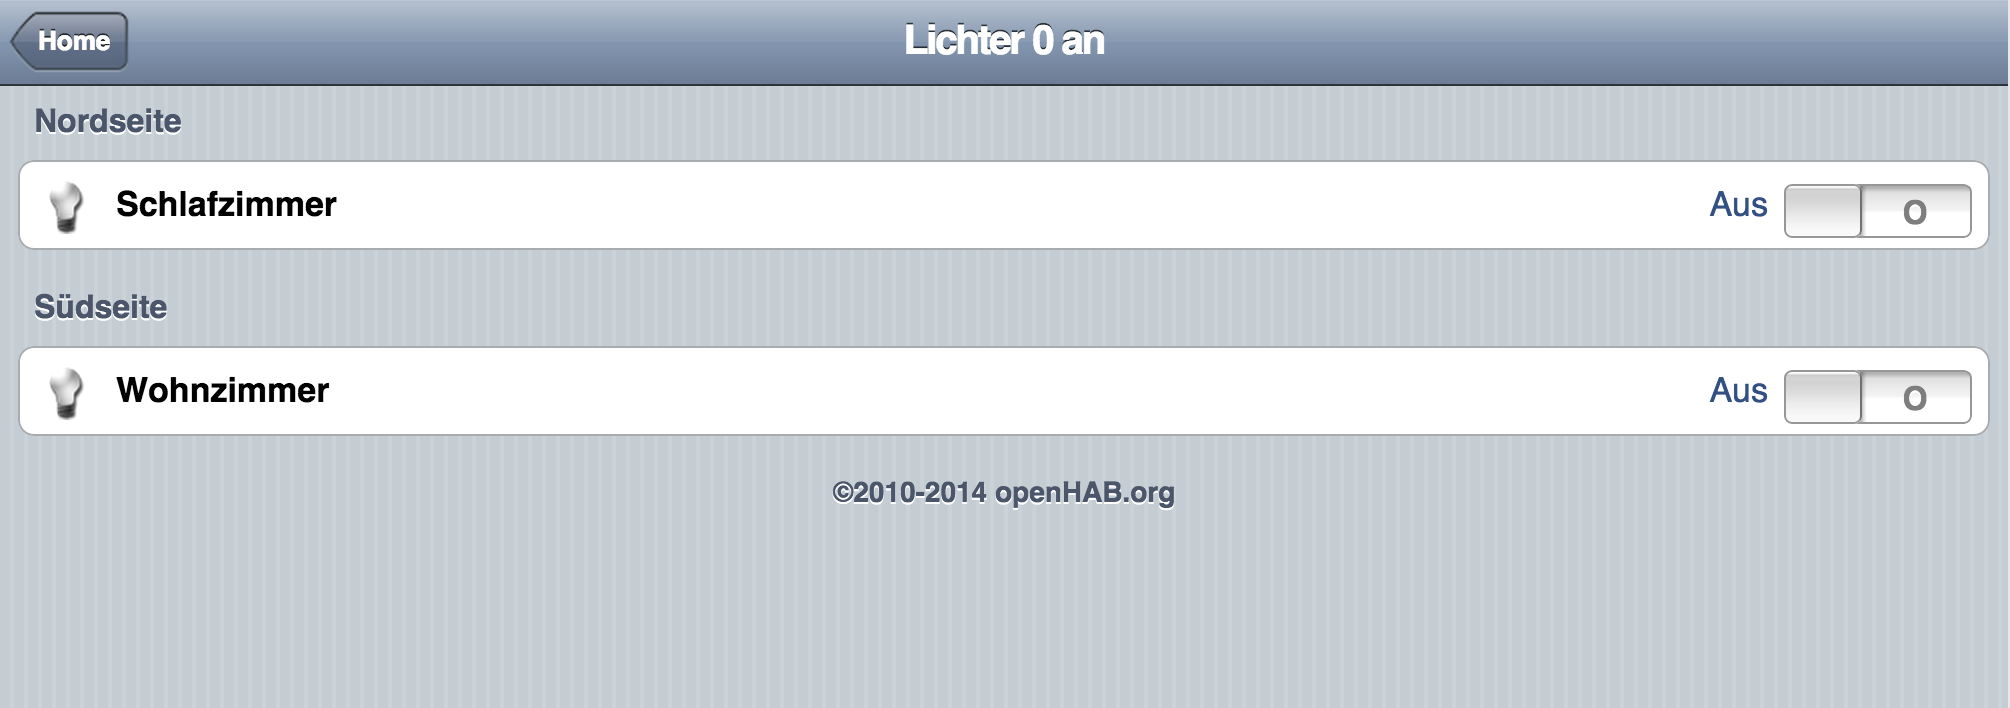
\includegraphics[scale=0.4]{appendix/img/standardGui}
	\caption{Web-GUI openHAB}
	\label{fig:guiOpenhab}
\end{figure}

\pagebreak
\section*{Zertifikat Erzeugen}
Die Zertifikate wurden mit OpenSSL (\url{http://slproweb.com/products/Win32OpenSSL.html}) erzeugt.

\subsection*{CA Zertifikat erstellen}
\lstinline!openssl req -new -x509 -days 3650 -keyout m2mqtt_ca.key -out m2mqtt_ca.crt! \\
Dieser Command erzeugt ein CA (Certificate Authority) Zertifikat mit einem privatem Schlüssel. Das X.509-Zertifikat ist für 3650 Tage gültig.

\subsection*{Server Zertifikat erstellen}
\lstinline!openssl genrsa -des3 -out m2mqtt_srv.key 1024! \\
Erzeugt einen 1024 Bit grossen 3DES, privaten Schlüssel. 

\subsection*{Signierung des Server Zertifikates}
\lstinline!openssl req -out m2mqtt_srv.csr -key m2mqtt_srv.key -new! \\
Dieses Kommando erzeugt ein Zertifikat-Request vom Server zur Signierung an die CA. Durch dieses Kommando wird lediglich der Request erzeugt. Das bedeutet, dass die Signierung noch nicht durchgeführt wurde.

\lstinline!openssl x509 -req -in m2mqtt_srv.csr -CA m2mqtt_ca.crt -CAkey m2mqtt_ca.key -CAcreateserial -out m2mqtt_srv.crt -days 3650!

Mit diesem Kommando wird der Server-Request signiert. Als Produkt entsteht das finale Zertifikat für den Broker.

Für die Client-Library (M2Mqtt) muss das Zertifikat noch ins DER-Format konvertiert werden: \\
\lstinline!openssl x509 -outform der -in m2mqtt_ca.crt -out m2mqtt_ca.der!

\pagebreak
\section*{Android App - Hawk Eye}
\label{sec:manualAndroidApp}
Diese Android App bietet einen Zugang zum openHAB System. Dadurch können die Status der verschiedenen Sensoren und Aktoren abgefragt werden. Ebenfalls kann über ein Schalter die einzelnen Glühbirnen ein- oder ausgeschaltet werden. Nachfolgend werden alle Screens gezeigt und erklärt.

\begin{figure}[htbp]
	\begin{minipage}{0.6\textwidth} 
Die Abbildung \ref{fig:screenshot_1} zeigt den Home-Screen. Durch Tippen auf «Einrichten» gelangt man zu den Einstellungen. Durch Tippen auf den Pfeil gelangt man zur Übersicht. Dies ist jedoch nur möglich, wenn die Verbindungseinstellungen korrekt sind und eine Verbindung zum openHAB hergestellt werden kann.
	\end{minipage}
	\hfill
	\begin{minipage}{0.32\textwidth}
		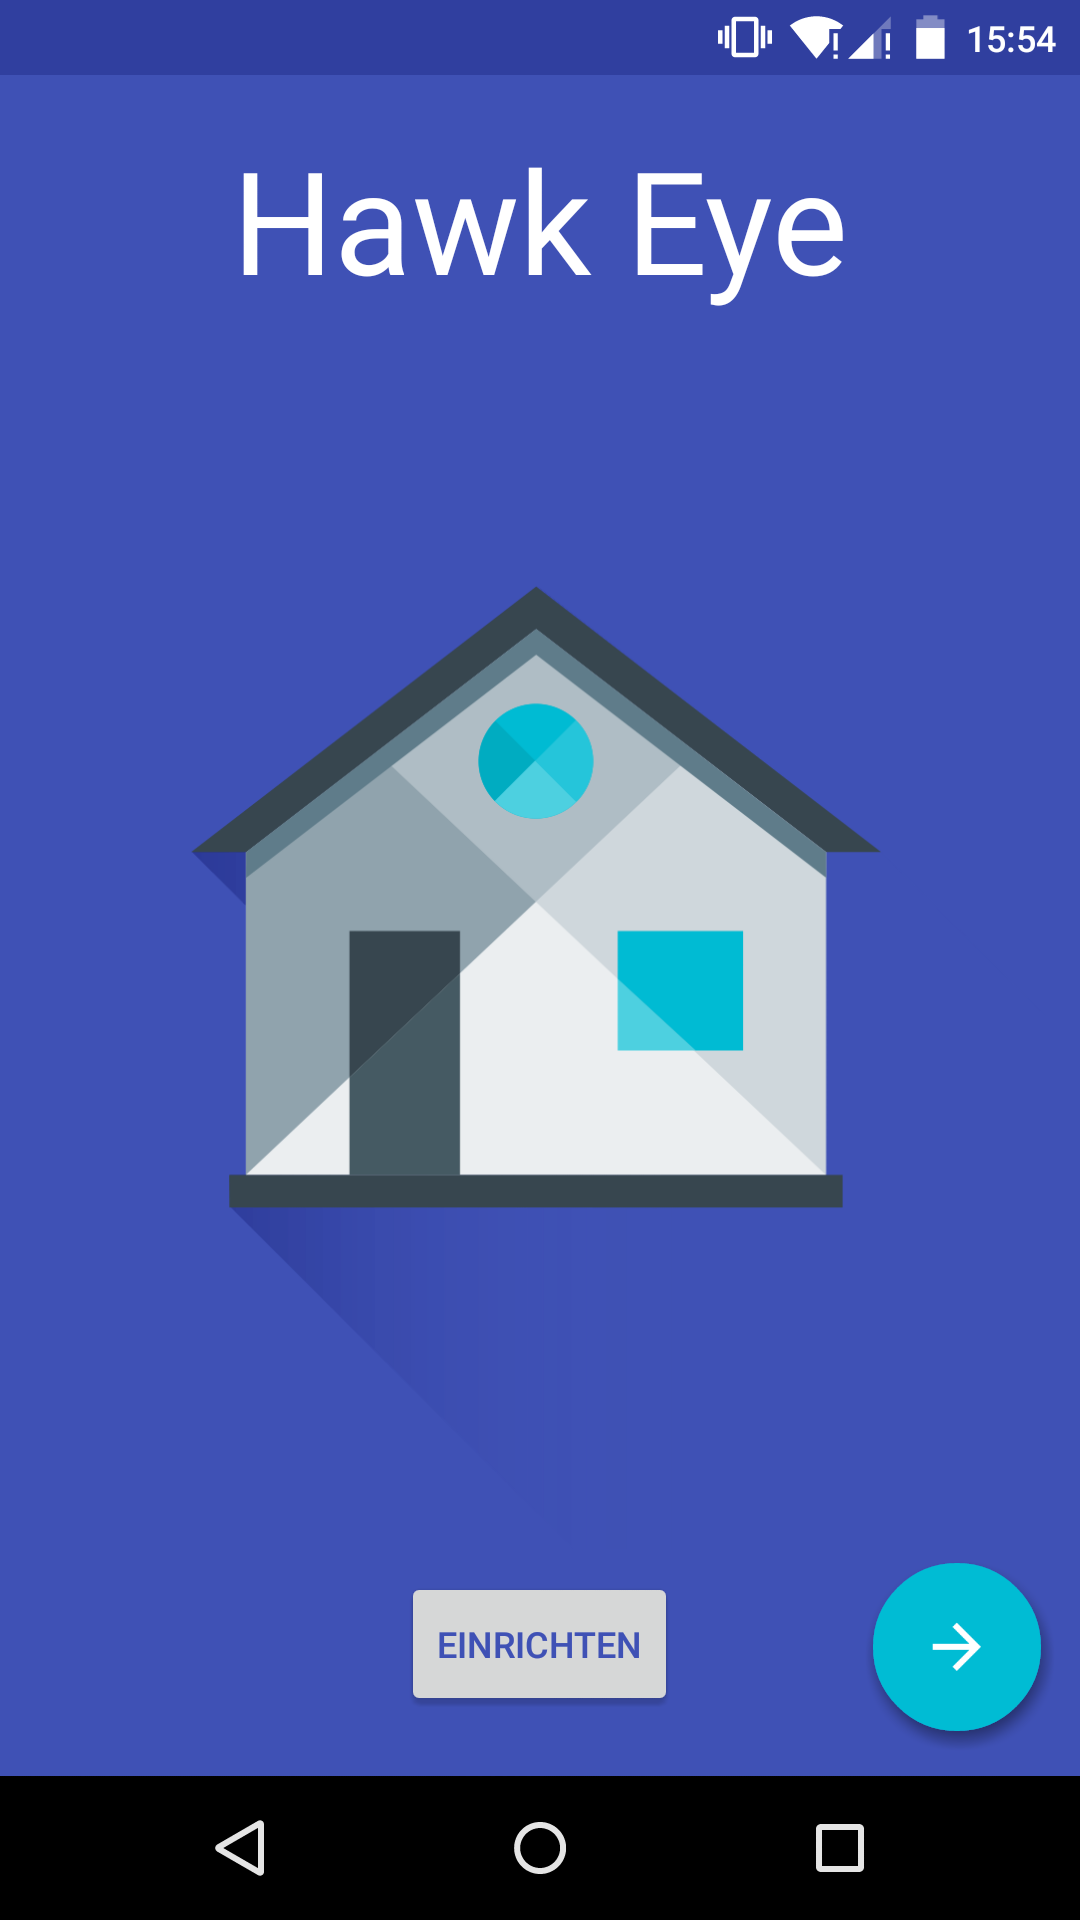
\includegraphics[scale=0.12]{appendix/img/AppScreenshots/Screenshot1}
		\caption{Start Screen}
		\label{fig:screenshot_1}
	\end{minipage}
\end{figure}

\begin{figure}[htbp]
	\begin{minipage}{0.6\textwidth} 
Die Abbildung \ref{fig:screenshot_2} zeigt die Einstellungen. Dazu muss die openHAB-URL (IP-Adresse des Raspberry Pis mit Port 8080) und der Name der Sitemap eingetragen werden. Durch Tippen auf «Verbindung Testen» können die Eingaben geprüft und die Konnektivität getestet werden. \\ \\
Des weiteren kann die Notification ein- und ausgeschaltet werden. Durch Tippen auf den Haken werden die Einstellungen gespeichert und die View geschlossen.
	\end{minipage}
	\hfill
	\begin{minipage}{0.32\textwidth}
		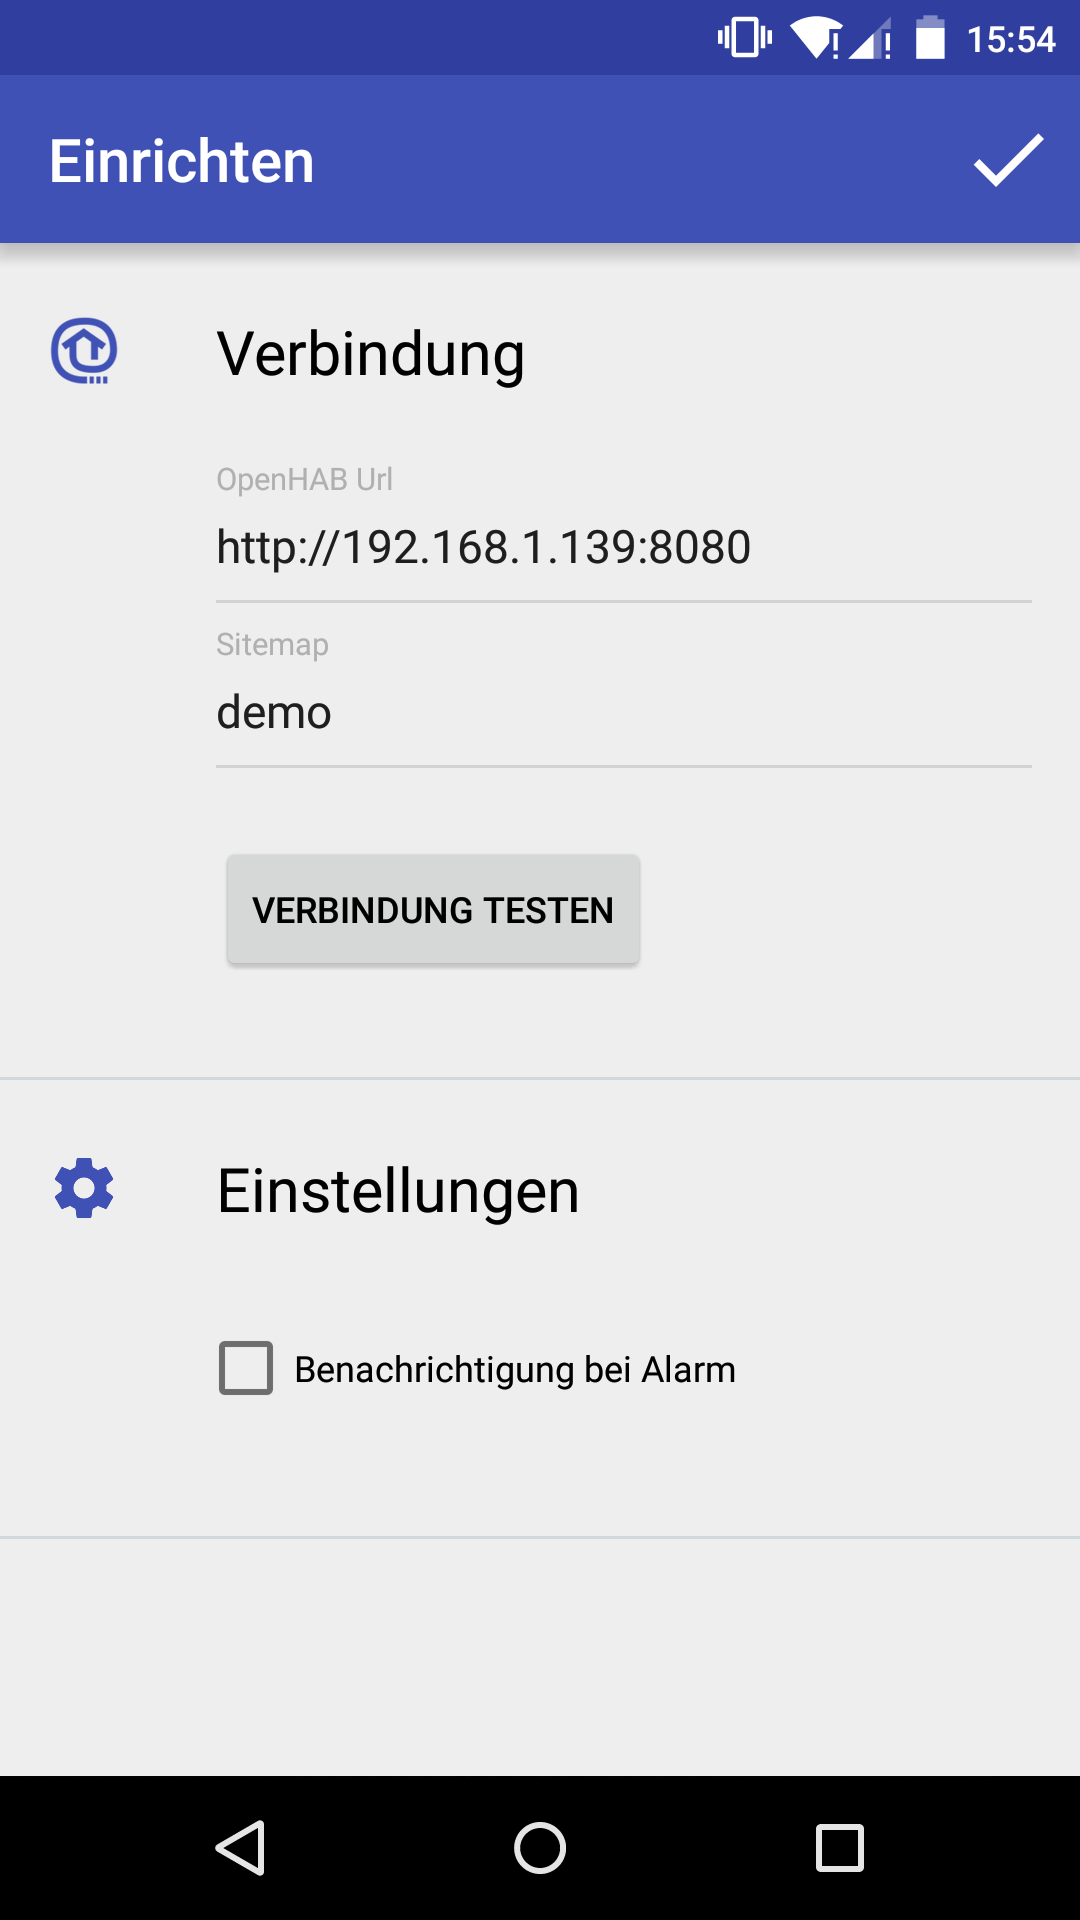
\includegraphics[scale=0.12]{appendix/img/AppScreenshots/Screenshot2}
		\caption{Config Screen}
		\label{fig:screenshot_2}
	\end{minipage}
\end{figure}


\begin{figure}[htbp]
	\begin{minipage}{0.6\textwidth} 
Wenn die Verbindungseigenschaften korrekt sind, wird das Sitemap dargestellt (Abbildung \ref{fig:screenshot_7}). Da sind die drei Bereiche zu sehen. Durch Tippen auf das Element gelangt man in die Detailansicht des entsprechenden Bereiches. Je nach Status wird dabei ein anderes Icon gezeigt. Falls zum Beispiel die Lichter ausgeschaltet sind, ändert die Farbe des Icons auf grau (inaktiv). \\ \\
In der Actionbar befindet sich rechts ein Zahnrad. Durch antippen dieses Symbols gelangt man zu den Einstellungen.
\\ \\
Um die Seite zu aktualisieren und die Status neu zu laden, kann mit dem Finger von oben nach unten gezogen werden (swipe).
	\end{minipage}
	\hfill
	\begin{minipage}{0.32\textwidth}
		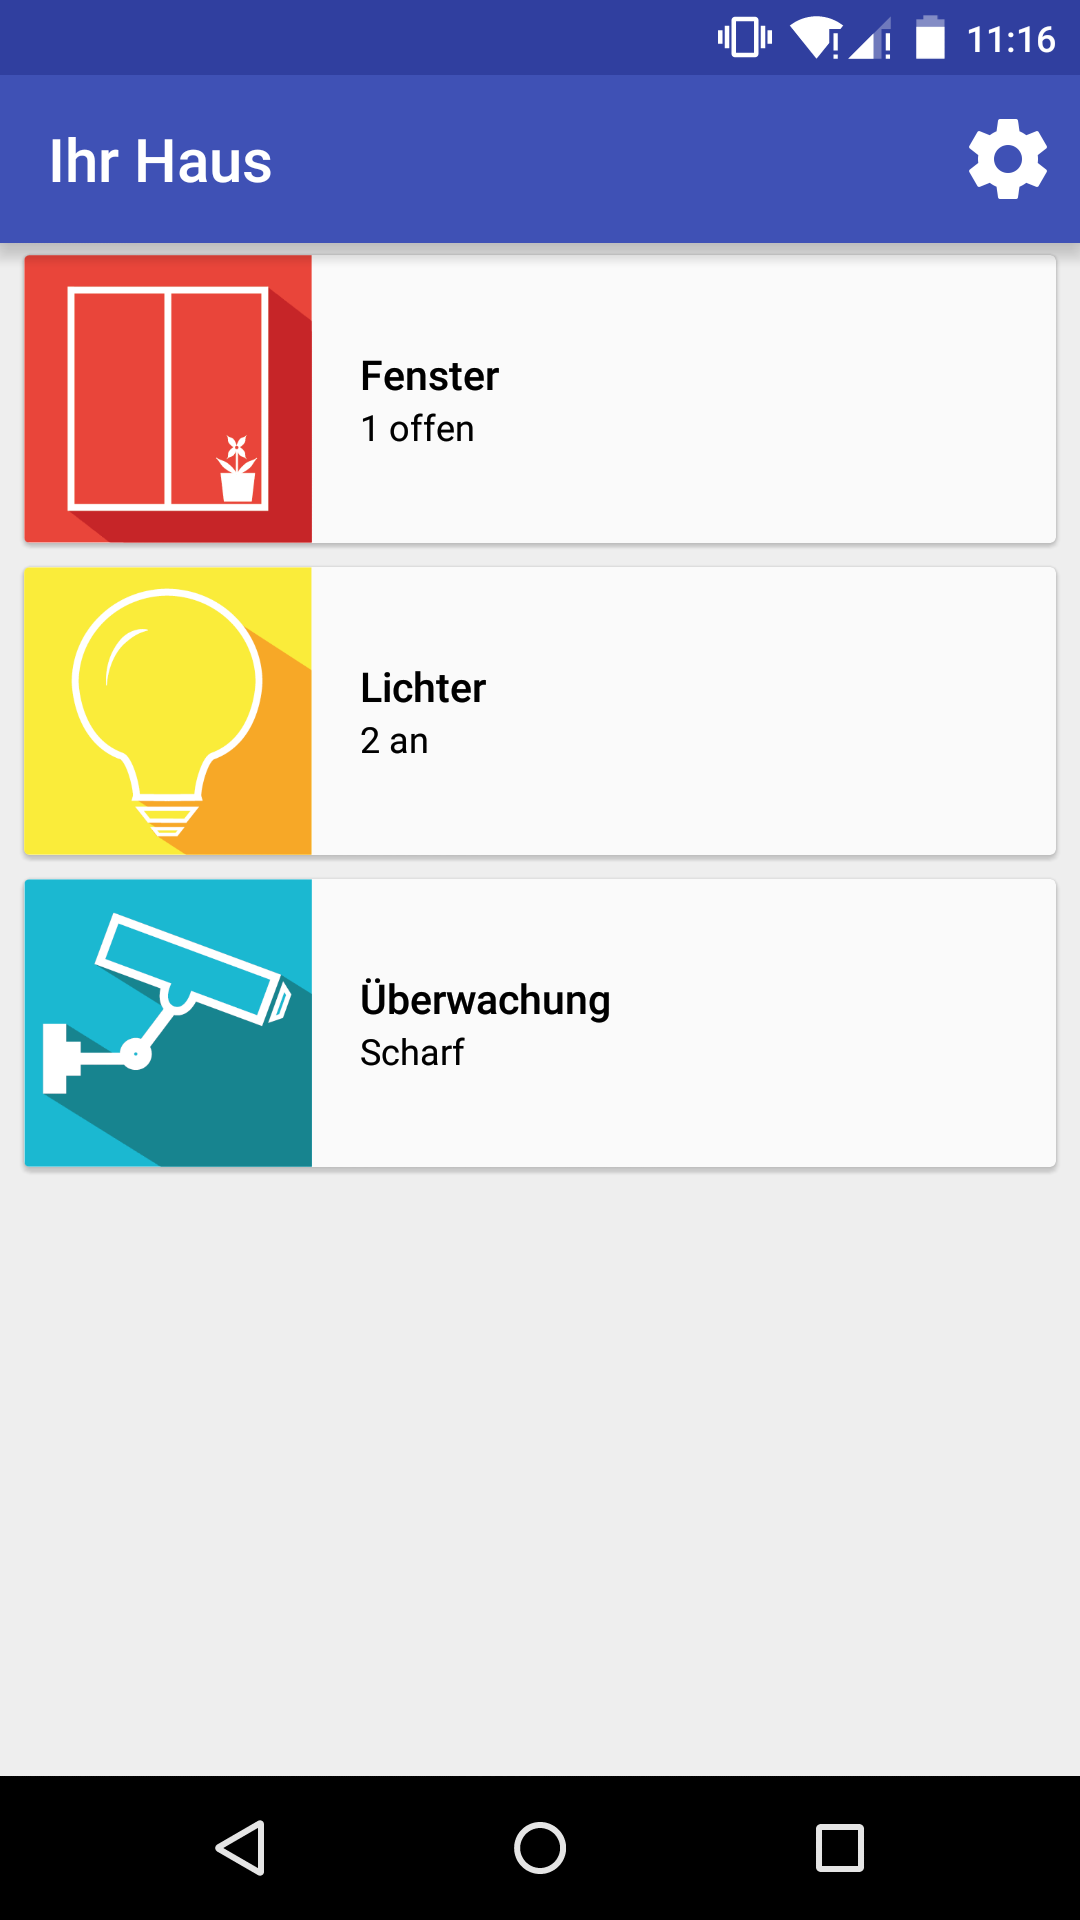
\includegraphics[scale=0.12]{appendix/img/AppScreenshots/Screenshot7}
		\caption{Alarm Beispiel}
		\label{fig:screenshot_7}
	\end{minipage}
\end{figure}


\begin{figure}[htbp]
	\begin{minipage}{0.6\textwidth} 
Diese Abbildung zeigt die Detailansicht des Bereiches «Fenster». Auch hier ändert sich jeweils das Icon, falls sich der Status des Items ändert (siehe Abbildung \ref{fig:screenshot_6}). Durch Tippen auf den Back-Button von Android, gelangt man zurück zur Übersicht.
	\end{minipage}
	\hfill
	\begin{minipage}{0.32\textwidth}
		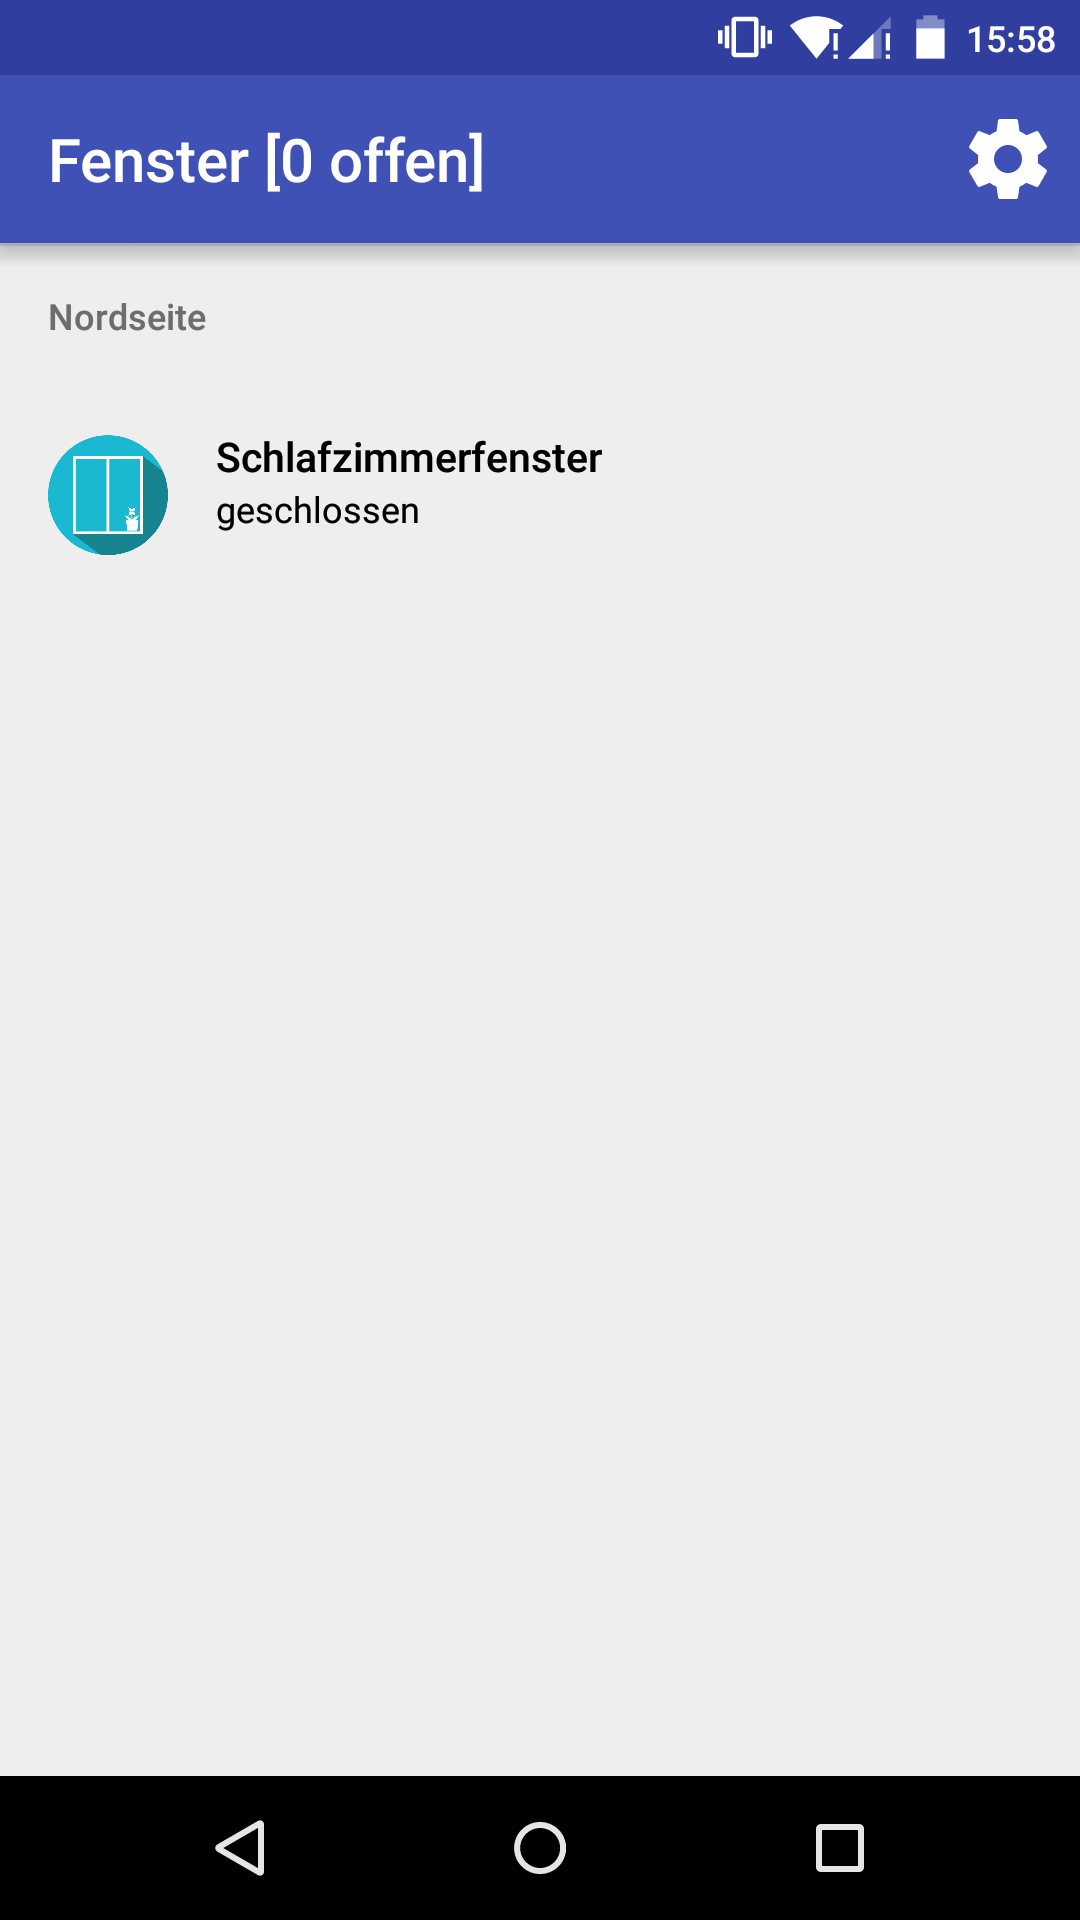
\includegraphics[scale=0.12]{appendix/img/AppScreenshots/Screenshot3}
		\caption{Window Item Screen}
		\label{fig:screenshot_3}
	\end{minipage}
\end{figure}

\begin{figure}[htbp]
	\begin{minipage}{0.6\textwidth} 
Das Icon ändert auf rot, wenn mindestens ein Fenster geöffnet wurde.
	\end{minipage}
	\hfill
	\begin{minipage}{0.32\textwidth}
		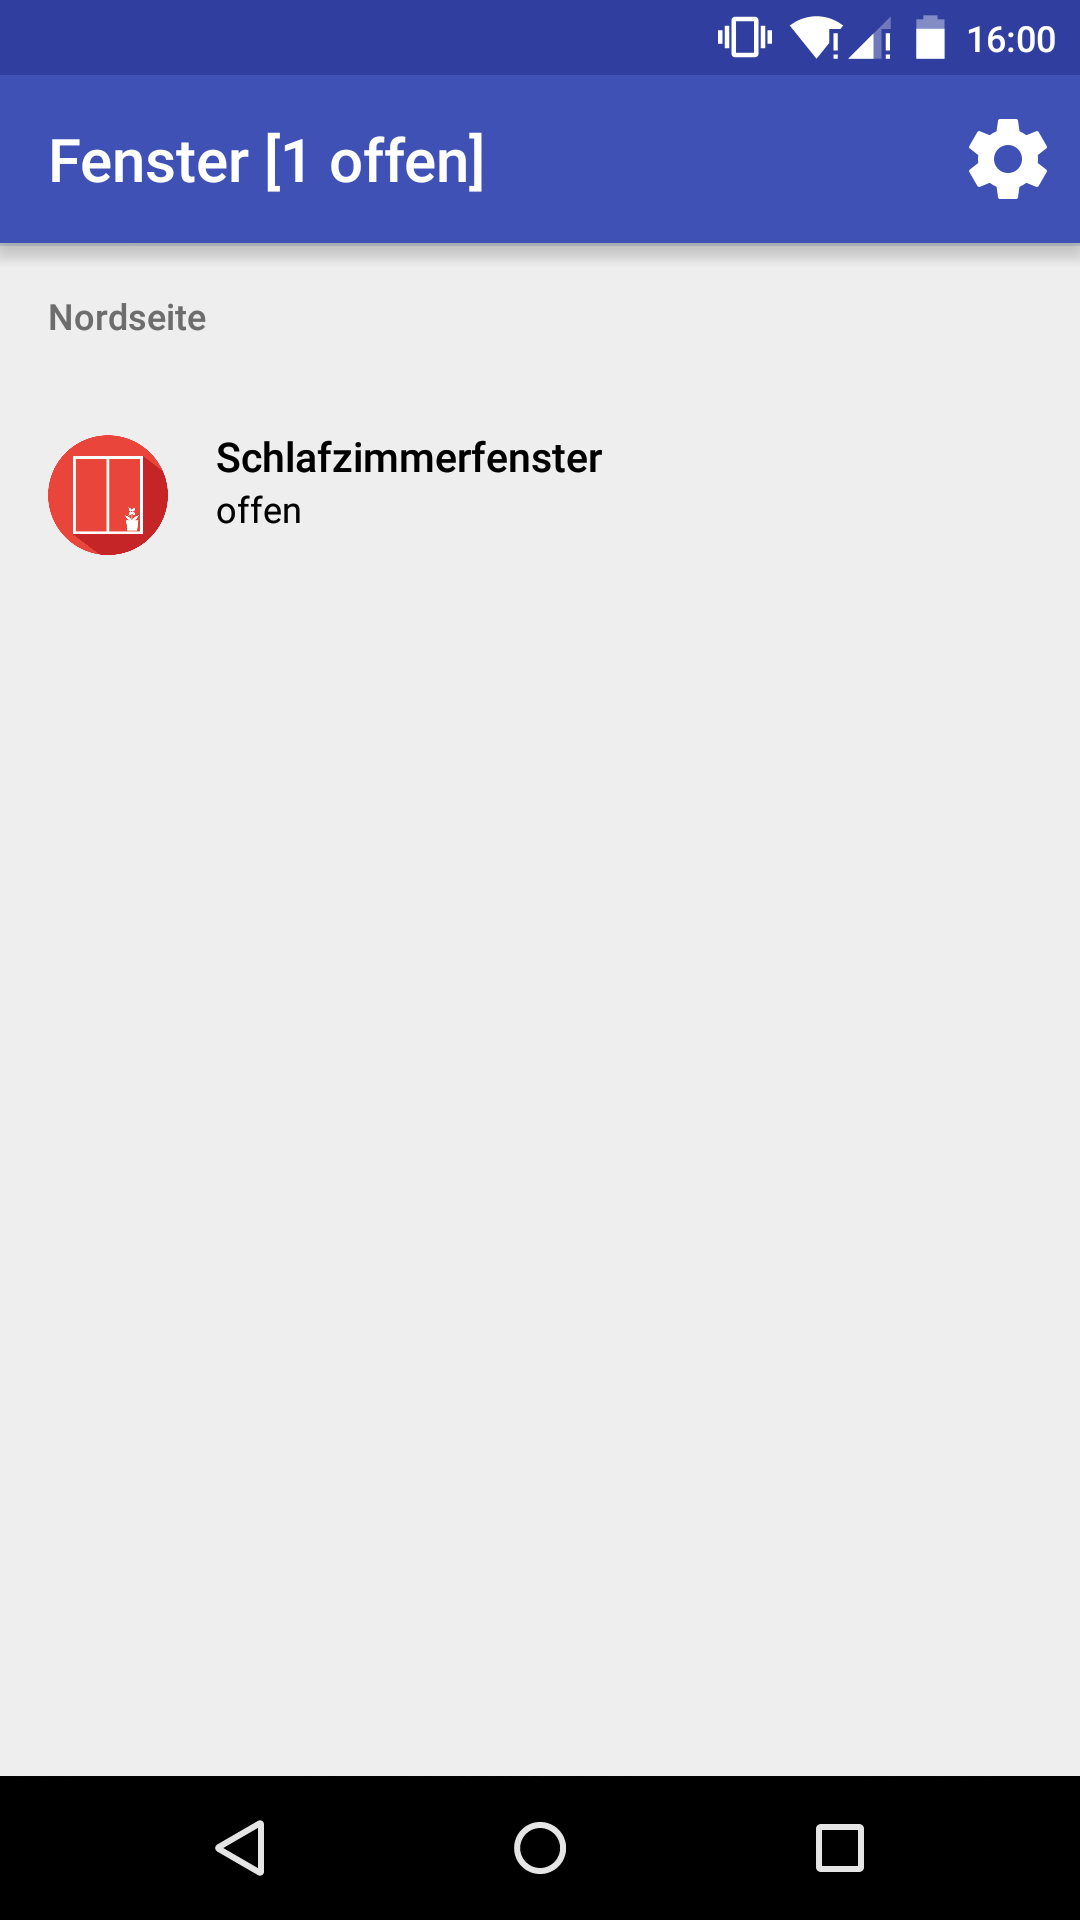
\includegraphics[scale=0.12]{appendix/img/AppScreenshots/Screenshot6}
		\caption{Alarm Item Beispiel}
		\label{fig:screenshot_6}
	\end{minipage}
\end{figure}

\begin{figure}[htbp]
	\begin{minipage}{0.6\textwidth} 
In der Abbildung \ref{fig:screenshot_4} wird die Detailansicht des Bereiches «Licht». Die einzelnen Lampen können über den Schalter ein- und ausgeschaltet werden. Je nach dem ändert sich auch hier das Icon.
	\end{minipage}
	\hfill
	\begin{minipage}{0.32\textwidth}
		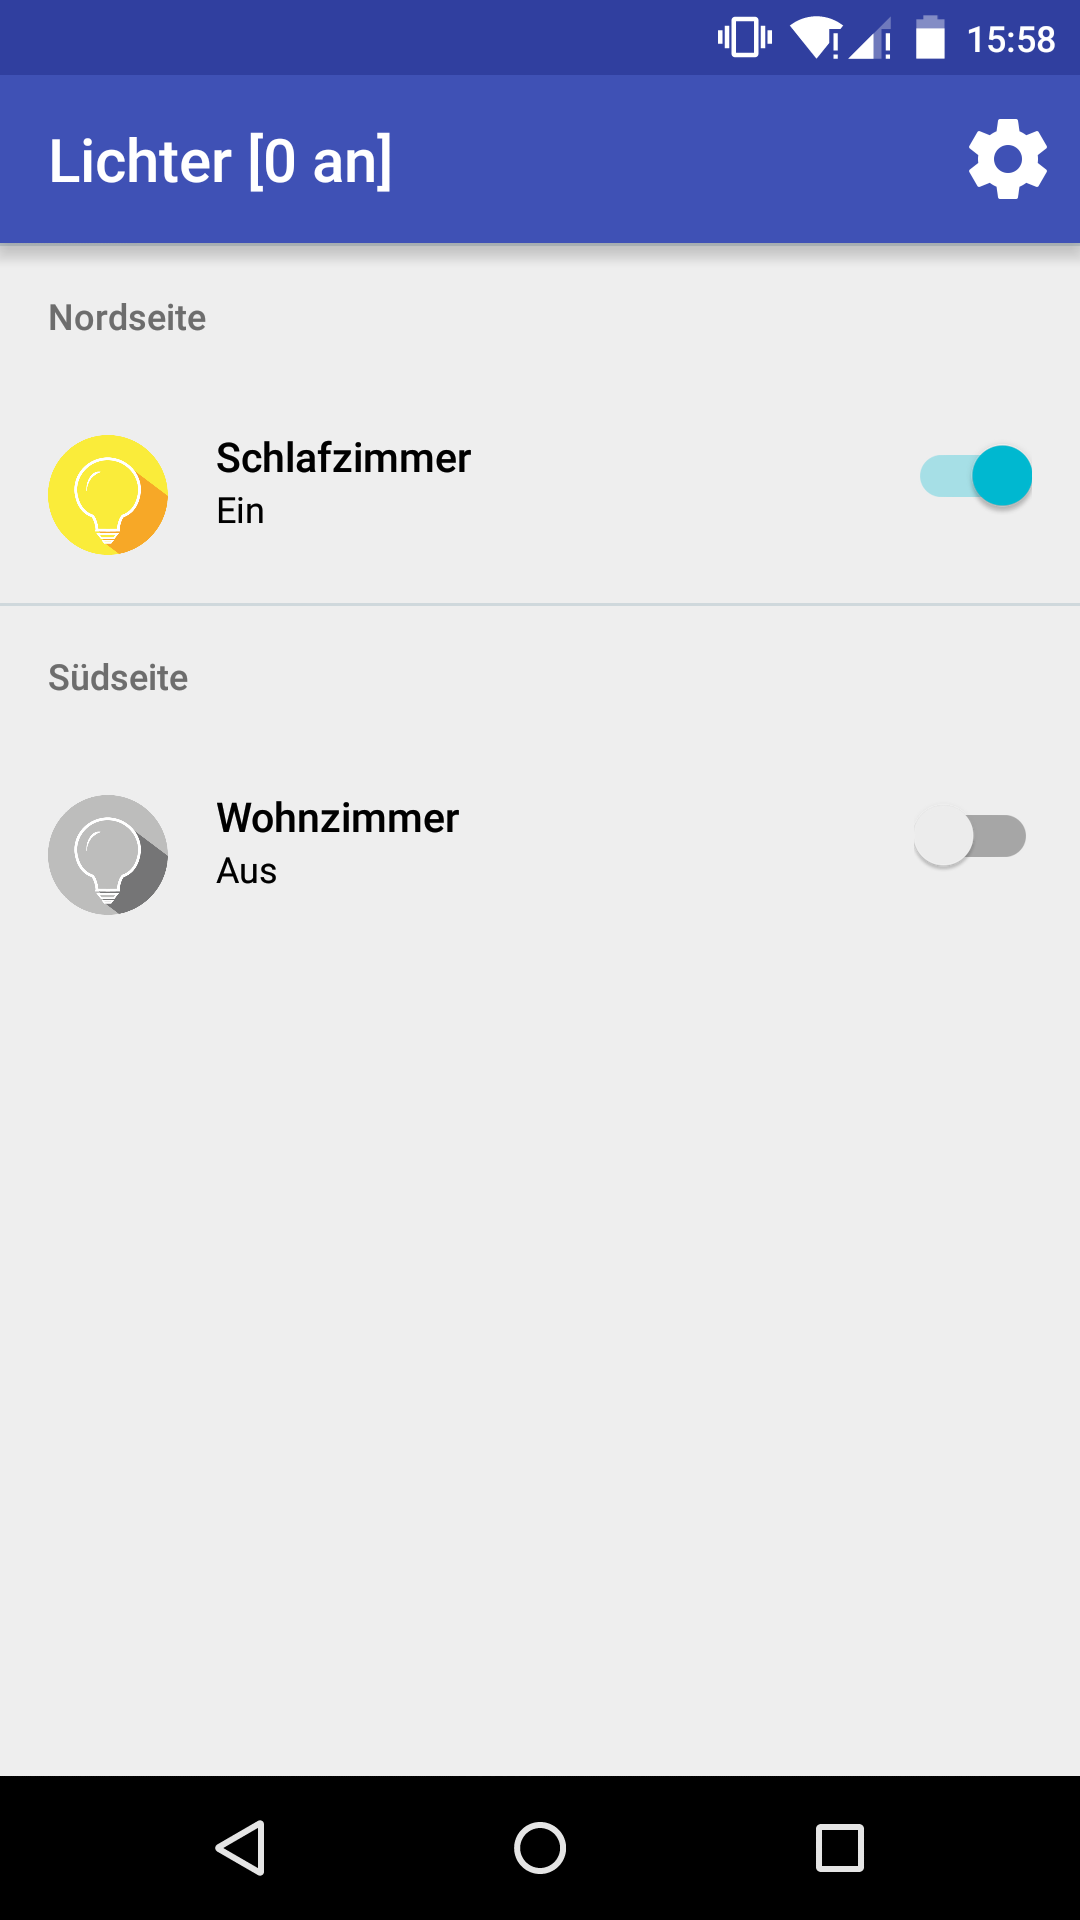
\includegraphics[scale=0.12]{appendix/img/AppScreenshots/Screenshot4}
		\caption{Light Item Screen}
		\label{fig:screenshot_4}
	\end{minipage}
\end{figure}

\begin{figure}[htbp]
	\begin{minipage}{0.6\textwidth} 
Der Bereich Überwachung ist das Kernstück der App. Hier kann die Alarmbereitschaft ein- und ausgeschaltet werden. Wenn der Alarm ausgeschaltet ist, wird man weder benachrichtigt, noch ändern sich die Icons, wenn sich ein Status ändert.\\
Weiter wird hier die Information gegeben, ob eine Bewegung detektiert wurde. \\ \\
Im unteren Bereich ist die Kamera zu sehen. Durch Scrollen sieht man das ganze Bild. 
	\end{minipage}
	\hfill
	\begin{minipage}{0.32\textwidth}
		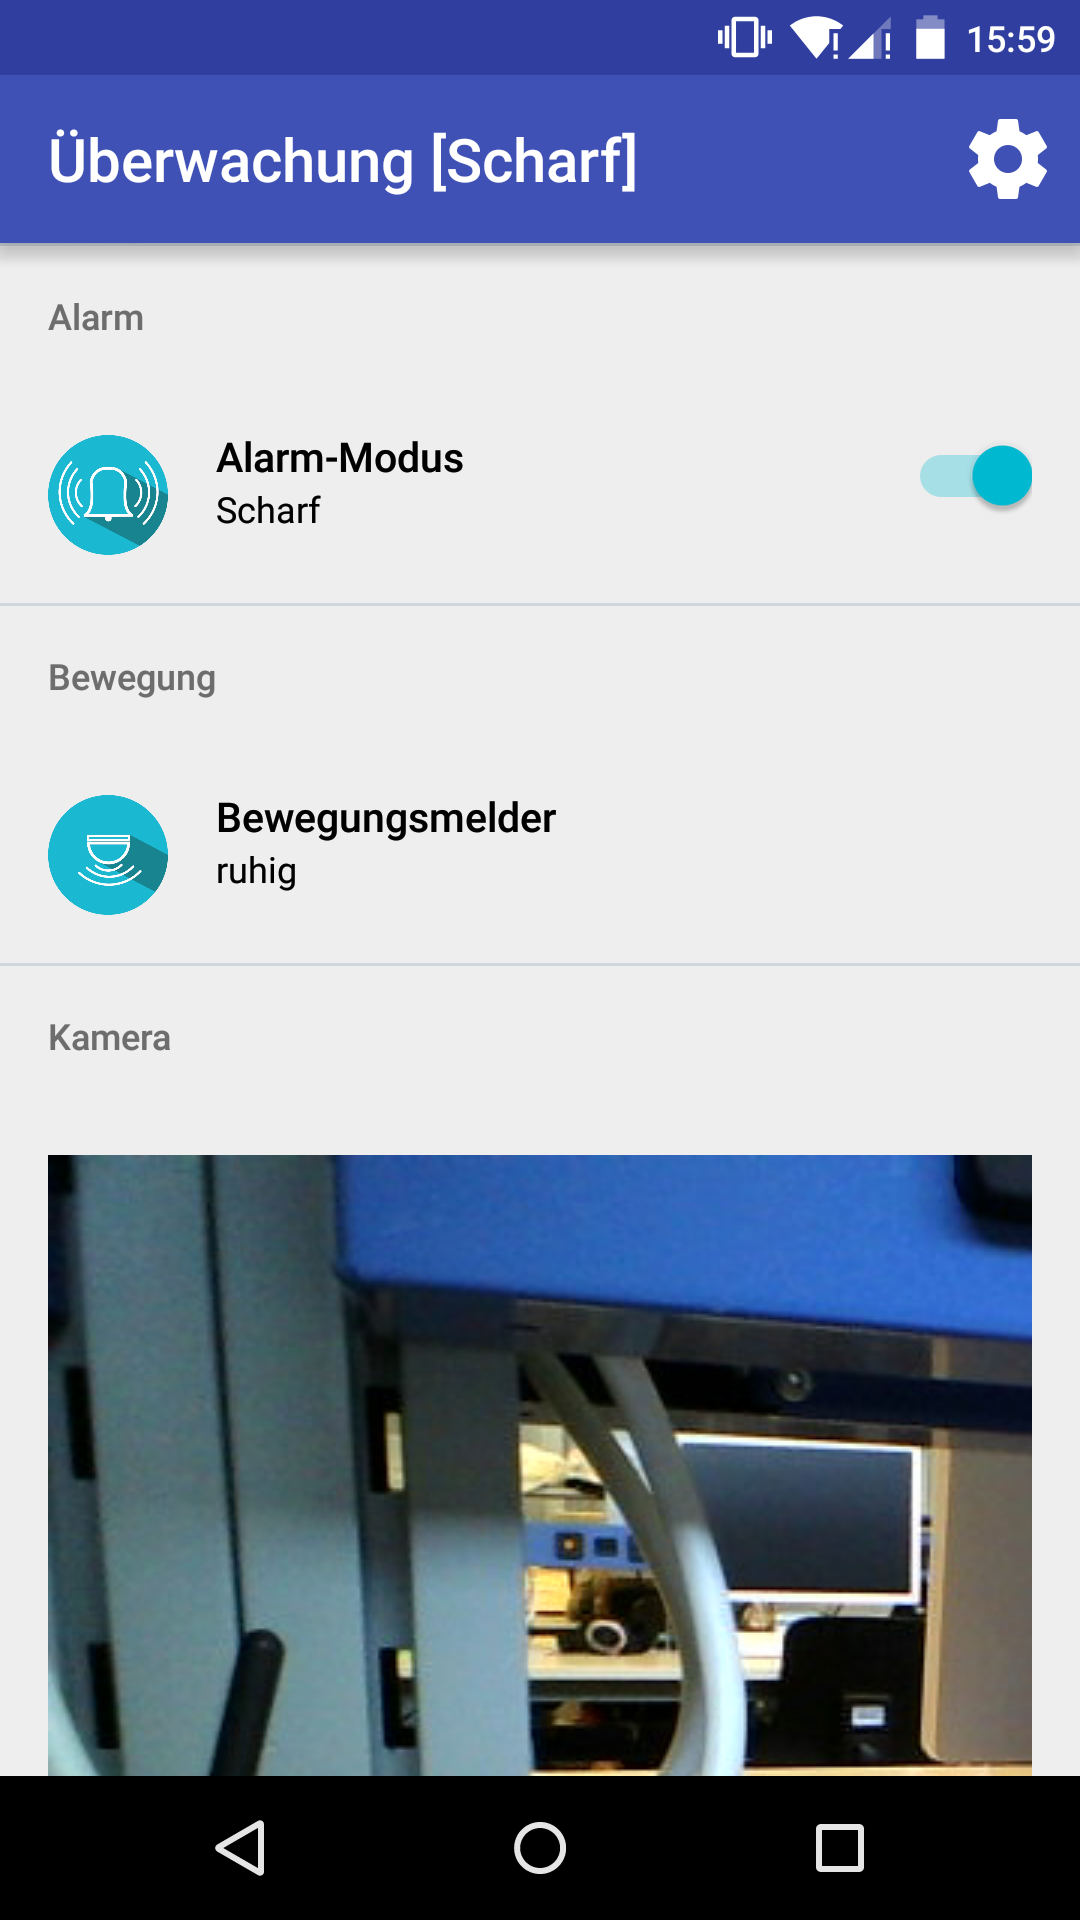
\includegraphics[scale=0.12]{appendix/img/AppScreenshots/Screenshot5}
		\caption{Monitoring Screen}
		\label{fig:screenshot_5}
	\end{minipage}
\end{figure}
